\documentclass[11pt,a4paper,fontset=fandol]{ctexart}
\usepackage[top=23mm,bottom=24mm,left=24mm,right=24mm]{geometry}
\usepackage{amsmath,amssymb,amsthm,bm,mathtools}
\usepackage{graphicx,booktabs,array,tabularx,multirow}
\usepackage[ruled,vlined,linesnumbered]{algorithm2e}
\SetAlgorithmName{算法}{算法}{算法目录}
\SetKwInput{KwIn}{输入}
\SetKwInput{KwOut}{输出}
\usepackage{enumitem,float,placeins,xcolor,fancyhdr}
\usepackage[numbers,sort&compress]{natbib}
\usepackage{url}
\usepackage[unicode,colorlinks=true,linkcolor=blue!45!black,citecolor=blue!45!black,urlcolor=blue!55!black]{hyperref}
\usepackage{microtype}
\setmainfont{TeX Gyre Termes}
\setmonofont{Latin Modern Mono}[Scale=0.86]
\linespread{1.12}
\raggedbottom
\setlength{\parskip}{0.25em}
\setlength{\emergencystretch}{2em}
\setlength{\headheight}{15pt}
\setlength{\textfloatsep}{12pt plus 3pt minus 2pt}
\setlength{\floatsep}{10pt plus 3pt minus 2pt}
\setlist[itemize]{leftmargin=1.7em,itemsep=0.12em,topsep=0.25em}
\setlist[enumerate]{leftmargin=2em,itemsep=0.12em,topsep=0.25em}
\pagestyle{fancy}
\fancyhf{}
\fancyhead[L]{\small Muon 优化算法的理论与仿真}
\fancyhead[R]{\small 优化与博弈课程大作业}
\fancyfoot[C]{\thepage}
\renewcommand{\headrulewidth}{0.3pt}
\ctexset{section={format=\Large\bfseries},subsection={format=\large\bfseries},subsubsection={format=\normalsize\bfseries}}
\newtheorem{assumption}{假设}[section]
\newtheorem{lemma}{引理}[section]
\newtheorem{theorem}{定理}[section]
\newtheorem{corollary}{推论}[section]
\theoremstyle{remark}
\newtheorem{remark}{说明}[section]
\renewcommand{\proofname}{证明}
\newcommand{\R}{\mathbb R}
\newcommand{\E}{\mathbb E}
\newcommand{\Frob}[1]{\left\lVert#1\right\rVert_F}
\newcommand{\op}[1]{\left\lVert#1\right\rVert_2}
\newcommand{\nuc}[1]{\left\lVert#1\right\rVert_*}
\newcommand{\inner}[2]{\left\langle#1,#2\right\rangle}
\newcommand{\polar}{\operatorname{polar}}
\newcommand{\CodeURL}{https://github.com/TrueEway/muon-course-project}
\newcommand{\ParameterCount}{112512}
\newcommand{\VocabSize}{65}
\newcommand{\TrainChars}{1003854}
\newcommand{\ValChars}{55769}
\newcommand{\TestChars}{55771}
\newcommand{\DataSHA}{86c4e6aa9db7c042ec79f339dcb96d42b0075e16b8fc2e86bf0ca57e2dc565ed}
\newcommand{\ResultDigest}{5fecfc7a11bdc5d2}
\newcommand{\MaxBoundRatio}{0.999990}
\newcommand{\MaxDescentViolation}{1.11e-16}
\newcommand{\AdamLR}{0.003}
\newcommand{\MuonSVDLR}{0.02}
\newcommand{\MuonNSLR}{0.05}
\newcommand{\AdamCE}{1.962}
\newcommand{\AdamPPL}{7.110}
\newcommand{\AdamTime}{20.710}
\newcommand{\SVDCE}{1.793}
\newcommand{\SVDPPL}{6.008}
\newcommand{\SVDTime}{28.504}
\newcommand{\NSCE}{1.843}
\newcommand{\NSPPL}{6.316}
\newcommand{\NSTime}{26.577}

\newcommand{\RevisionDigest}{dc216a9cf99f21ec}
\newcommand{\CifarBestValK}{7}
\newcommand{\CifarSGDAcc}{63.12}
\newcommand{\CifarSGDStep}{9.3}
\newcommand{\CifarSGDWall}{31.1}
\newcommand{\CifarAdamAcc}{69.21}
\newcommand{\CifarAdamStep}{9.9}
\newcommand{\CifarAdamWall}{33.1}
\newcommand{\CifarMuonAcc}{74.57}
\newcommand{\CifarMuonStep}{26.8}
\newcommand{\CifarMuonWall}{85.9}
\newcommand{\CifarMuonSpeed}{1.00}

\graphicspath{{../output/figures/}}
\title{\vspace{-1.2em}\bfseries Muon 优化算法\\[0.25em]\Large 矩阵更新机制、随机非凸收敛分析与仿真研究}
\author{优化与博弈课程大作业}
\date{2026 年 11 月}
\hypersetup{pdftitle={Muon优化算法：矩阵更新机制、随机非凸收敛分析与仿真研究},pdfauthor={}}

\begin{document}
\maketitle
\thispagestyle{empty}
\begin{abstract}
Muon 对动量矩阵作近似极分解后更新参数，利用谱范数与核范数的对偶关系保留矩阵方向结构。本文完整推导精确版本的确定性与随机非凸收敛界，并补充一个显式含谱范数近似误差 $\delta$ 的条件定理：若全程误差统一小于 1，在 $\eta=\Theta(T^{-3/4})$、$1-\beta=\Theta(T^{-1/2})$ 的调度下，平均期望梯度核范数为 $O(T^{-1/4})$。同时说明固定五步多项式并不自动满足该全程误差假设。实验新增条件数 $10^4$ 的非凸矩阵分解、完整 ResNet-18 的 CIFAR-10 比较，以及 $K=0,1,3,5,7$ 的三种子训练消融。SGD+M、AdamW 与五步 Muon 混合的选定测试准确率分别为 \CifarSGDAcc\%、\CifarAdamAcc\% 与 \CifarMuonAcc\%；Muon 相对于 SGD 的验证阈值配对步数比为 \CifarMuonSpeed。图表同时报告更新谱、单步活跃时间和显存开销，未达阈值时保留未达标记录。新实验采用固定预算，原始日志、绘图入口和分章节源码见\href{https://github.com/TrueEway/muon-course-project/tree/v1.1}{公开代码仓库}。
\end{abstract}
\noindent\textbf{关键词：} Muon；极分解；谱范数；随机非凸优化；动量；Newton--Schulz

\section{引言与相关研究}
\subsection{研究问题}
神经网络训练通常写成随机优化问题
\begin{equation}\label{eq:problem}
 \min_{\theta} f(\theta)=\E_{\xi}[\ell(\theta;\xi)].
\end{equation}
其中 $\xi$ 表示一个样本或一个小批量。对大模型而言，优化器不仅决定每一步向哪个方向移动，也会改变状态存储、更新计算量以及训练稳定性。一个每步更复杂的算法可能减少达到目标损失所需的步数，也可能因为更新成本较高而增加实际训练时间。因此，比较优化器时至少需要区分迭代效率与时间效率。

SGD 使用当前小批量梯度更新参数，动量 SGD 则把历史梯度纳入更新方向。在此基础上，Adam 用逐坐标一阶、二阶矩估计调整步长\citep{adam2015}；AdamW 进一步把权重衰减从梯度统计中分离\citep{adamw2019}。这类方法可以处理不同形状的参数，但其基本归一化操作以坐标为单位。神经网络中的线性层权重本来是矩阵，将其视为一个长向量，会弱化输入方向、输出方向及奇异值谱所包含的结构。

Muon 采用另一种做法：先计算动量，再对动量矩阵作近似正交化，最后更新参数\citep{jordan2024}。在精确极分解的理想情况下，所有非零奇异值都被替换为 1，而奇异向量保持不变。更新不再由最大奇异值方向单独支配。不过，这并不直接说明算法必然优于 AdamW：方向归一化同时丢弃幅度信息，噪声可能影响小奇异值方向，近似正交化也有计算成本。

本文围绕三个问题展开：第一，Muon 更新在什么意义下是最速下降方向？第二，在动量与随机梯度同时存在时，可以证明什么收敛结论？第三，在受控矩阵实验与完整 ResNet-18 图像实验中，理论界、精确更新和有限步实现分别表现如何？这三个问题对应几何解释、数学证明和实验检验，而非对所有模型作统一的优劣排序。

\subsection{文献脉络与本文定位}
Bernstein 与 Newhouse\citep{bernstein2024} 从不同范数下的最速下降解释优化算法，为理解矩阵更新提供了直接入口。Cutkosky 与 Mehta\citep{cutkosky2020} 分析归一化随机梯度中的动量作用，说明动量跟踪误差可以成为收敛证明的核心变量。矩阵问题还需要处理谱范数与核范数的对偶关系，以及从核范数误差到 Frobenius 范数误差时出现的维度因子。

早期 Muon 收敛分析\citep{lihong2025} 已讨论精确 SVD 版本，但某些中间不等式需要谨慎核查。后续工作\citep{chang2025} 明确讨论了已有证明的问题，并进一步分析不同动量和方差缩减版本。本文不以早期论文中含矩阵逆的推导为证明依据，而是从范数对偶关系重新组织一条可逐步检查的证明。所得阶数属于已有理论框架的课程性推导，不声称为新的收敛率。

在应用方面，Liu 等\citep{liu2025} 研究了 Muon 向大模型训练扩展时的权重衰减与更新尺度问题。有限步 Newton--Schulz 与 Nesterov 修正的直接分析也已有专门研究\citep{peng2026}。这些工作提醒我们：精确极分解、有限多项式迭代和带其他参数组的混合实现并非同一个数学迭代。报告中必须明确区分。

本文的工作包括：给出处理零矩阵和秩亏情形的精确更新定义；证明精确版本与含谱范数近似误差版本的有限步平均梯度界；在独立调参后比较病态非凸矩阵分解与完整 ResNet-18；用真实更新谱和 $K$ 消融检查近似机制及计算开销。原有受控二次问题、随机梯度和语言模型实验保留在附录。所有数值表格都由运行记录生成，代码入口与数据校验值在第\ref{sec:reproduce}节给出。

\section{数学准备与算法描述}
\subsection{矩阵范数与精确极因子}
对 $W\in\R^{m\times n}$，记 $r=\min(m,n)$。本文使用 Frobenius 内积
$\inner{A}{B}=\operatorname{tr}(A^\top B)$，并区分三个范数：
\begin{equation}
 \Frob{A}=\Bigl(\sum_i s_i(A)^2\Bigr)^{1/2},\quad
 \op{A}=s_1(A),\quad \nuc{A}=\sum_i s_i(A).
\end{equation}
由 Cauchy--Schwarz 不等式，$\Frob{A}\leq\nuc{A}\leq\sqrt r\Frob{A}$。后一个关系中的 $\sqrt r$ 是本报告随机收敛常数出现维度依赖的来源，不能在隐藏常数时忽略。

若 $M=U_q\Sigma_qV_q^\top$ 为仅包含正奇异值的紧致 SVD，定义
\begin{equation}\label{eq:polar}
 O^\star=\polar(M)=U_qV_q^\top;\qquad \polar(0)=0.
\end{equation}
当 $M$ 满列秩或满行秩时，$O^\star$ 是半正交矩阵。秩亏时，$O^\star$ 是对应支撑子空间上的部分等距映射；一般不能写 $(O^\star)^\top O^\star=I$。这一约定与保留零奇异值对应基向量的任意半正交补全不同，但均可成为谱范数单位球上的线性子问题解。紧致约定能保证零动量不产生更新，也与多项式迭代对零奇异值的处理一致。

\begin{lemma}[对偶关系与方向性质]\label{lem:duality}
对任意矩阵 $M$，式\eqref{eq:polar}中的 $O^\star$ 满足
\begin{equation}\label{eq:dual}
 \op{O^\star}\leq1,\qquad \Frob{O^\star}\leq\sqrt r,\qquad
 \inner{M}{O^\star}=\nuc M=\max_{\op D\leq1}\inner M D.
\end{equation}
\end{lemma}
\begin{proof}
由紧致 SVD，$O^\star$ 的非零奇异值均为 1，数量为 $q\leq r$，故前两个结论成立。迹的循环性质给出 $\inner{M}{O^\star}=\operatorname{tr}(\Sigma_q)=\nuc M$。另一方面，von Neumann 迹不等式给出
$\inner M D\leq\sum_i s_i(M)s_i(D)\leq\nuc M\op D$，故任何可行 $D$ 的目标值都不超过 $\nuc M$。零矩阵情形直接成立。
\end{proof}

因此，$-O^\star$ 解决谱范数单位球上的线性最小化子问题，即
\begin{equation}
 \arg\min_{\|D\|_2\leq1}\inner{M}{D}\ \ni\ -O^\star.
\end{equation}
负号不能省略；$O^\star$ 本身最大化该内积。还需区分\emph{归一化方向}与\emph{局部二次模型的完整最优步}：
\begin{equation}\label{eq:quadraticmodel}
 \arg\min_D\left\{\inner M D+\frac{1}{2\gamma}\op D^2\right\}
 \ \ni\ -\gamma\nuc M\,O^\star.
\end{equation}
这是因为固定 $\op D=s$ 时，最小线性项为 $-s\nuc M$，再对 $s\geq0$ 最小化即可。Muon 使用的是 $-\eta O^\star$；不能把它与式\eqref{eq:quadraticmodel}在同一个数值步长下混为一谈。

\subsection{用于证明的精确版本}
记 $G_t$ 为在当前参数 $W_t$ 处取得的批量随机梯度，$\alpha=1-\beta$。本文理论版本如下。
\begin{algorithm}[htbp]
\caption{精确极因子 Muon：本文的理论分析对象}\label{alg:exact}
\KwIn{$W_1$，迭代预算 $T$，步长 $\eta>0$，动量参数 $0\leq\beta<1$，批量 $B$}
在 $W_1$ 处采样 $G_1$，初始化 $M_1\leftarrow G_1$\;
\For{$t=1,\ldots,T$}{
 \If{$t\geq2$}{在 $W_t$ 处采样 $G_t$\;
 $M_t\leftarrow\beta M_{t-1}+(1-\beta)G_t$\;}
 $O_t^\star\leftarrow\polar(M_t)$，零矩阵按式\eqref{eq:polar}处理\;
 $W_{t+1}\leftarrow W_t-\eta O_t^\star$\;
}
\KwOut{参数序列；用于理论评价时，均匀抽取一个 $W_t$}
\end{algorithm}

这里采用 $M_1=G_1$，便于明确初始误差；它与常见实现中从零缓冲区开始的约定不同。附录中的确定性二次问题与随机矩阵实验遵循算法\ref{alg:exact}。该版本没有偏差修正、权重衰减、梯度裁剪或 Nesterov 外推。

\subsection{有限步实现与参数分组}
实际实现先形成 EMA 动量 $M_t=\beta M_{t-1}+(1-\beta)G_t$，再可选地使用
\begin{equation}\label{eq:nesterov}
 N_t=\beta M_t+(1-\beta)G_t.
\end{equation}
该式采用参考代码的 EMA 插值约定。令 $X_0=N_t/(\Frob{N_t}+10^{-7})$，对较长维度作转置以降低矩阵乘法成本，再执行
\begin{equation}\label{eq:ns}
 X_{j+1}=aX_j+(bX_jX_j^\top+c(X_jX_j^\top)^2)X_j,
 \quad (a,b,c)=(3.4445,-4.7750,2.0315).
\end{equation}
最后转回原形状。本文五步配置采用 $j=0,\ldots,4$；历史 CPU 语言模型与新增 CUDA 图像实验均使用 float32，参考实现的 bfloat16 版本与此存在精度差异。若 $X_0=U\Sigma V^\top$，一次迭代保留奇异向量，并将奇异值映射为 $\phi(s)=as+bs^3+cs^5$。

有限步输出不必等于 $UV^\top$。经验系数的目标是用少量矩阵乘法获得有效方向，并不保证对任意谱，迭代越多就越接近精确极因子。$\phi(0)=0$ 也说明多项式本身不会补出缺失的秩。

应用更新为
\begin{equation}\label{eq:practical}
 W_{t+1}=(1-\eta_t\lambda)W_t-\eta_t s_{m,n}O_t,
 \qquad s_{m,n}=\sqrt{\max(1,m/n)}.
\end{equation}
语言模型只把 Transformer 块内的二维线性层权重分给 Muon。词嵌入、位置嵌入、输出层权重、偏置及归一化参数采用 AdamW。精确 SVD 对照也保留式\eqref{eq:nesterov}、形状缩放及相同参数分组，仅替换正交化方式。

新增 ResNet-18 实验将隐藏卷积核展平为“输出通道 $\times$ 其余维度”的二维矩阵。输入 stem、分类 head 和一维参数仍由 AdamW 更新。$K=0$ 消融定义为仅保留前置 Frobenius 归一化、不执行多项式；它不是零更新，也不等于未经归一化的 SGD 动量。
\begin{algorithm}[htbp]
\caption{实际混合 Muon 的参数分组与更新}\label{alg:hybrid}
\KwIn{隐藏矩阵组 $\mathcal H$，辅助组 $\mathcal A$，$K$，动量 $\beta$，步长与衰减}
初始化各隐藏参数的动量缓冲区为零\;
\For{每个训练批量}{
 在同一组当前参数处完成前向、反向，取得全部梯度\;
 \For{$W\in\mathcal H$}{
 将卷积梯度按输出通道展平，$M\leftarrow\beta M+(1-\beta)G$\;
 $N\leftarrow\beta M+(1-\beta)G$，$O\leftarrow\mathrm{NS}_K(N)$\;
 $W\leftarrow(1-\eta\lambda)W-\eta\sqrt{\max(1,m/n)}\,\mathrm{reshape}(O)$\;
 }
 对 $\mathcal A$ 执行一次 AdamW 更新，偏置及归一化参数不衰减\;
}
\end{algorithm}

对稠密 $m\times n$ 矩阵，薄 SVD 的典型算术量为 $O(mnr)$；转置后使用较小 Gram 矩阵的 $J$ 步多项式也为 $O(Jmnr)$，但具体常数、并行方式及数值精度不同。AdamW 的逐坐标更新为 $O(mn)$，通常保存两个矩估计；Muon 的矩阵参数部分仅持久保存一个动量矩阵，但正交化仍需临时工作空间。因此，状态数量较少与单步更新更快是两个不同的问题。


\FloatBarrier

\section{收敛性结果与完整证明}\label{sec:theory}
\subsection{假设、随机信息与评价指标}
以下只分析算法\ref{alg:exact}。令 $H_t=\nabla f(W_t)$，$Z_t=G_t-H_t$，$E_t=M_t-H_t$。用 $\mathcal F_t$ 表示采样 $G_t$ 之前已知的全部信息，其中包括 $W_t$ 和过去的样本。

\begin{assumption}[下界与光滑性]\label{ass:smooth}
存在有限 $f_{\inf}$，使 $f(W)\geq f_{\inf}$。对任意 $X,Y$，有
\begin{equation}\label{eq:smooth}
 \Frob{\nabla f(X)-\nabla f(Y)}\leq L\Frob{X-Y},\qquad L>0.
\end{equation}
记 $\Delta=f(W_1)-f_{\inf}$，初值 $W_1$ 固定。
\end{assumption}

\begin{assumption}[条件无偏与方差]\label{ass:noise}
对每个 $t$，批量梯度满足
\begin{equation}\label{eq:noise}
 \E[Z_t\mid\mathcal F_t]=0,\qquad
 \E[\Frob{Z_t}^2\mid\mathcal F_t]\leq\sigma^2/B.
\end{equation}
\end{assumption}

若每个样本的条件方差不超过 $\sigma^2$ 且同一批中的样本条件独立，则平均梯度满足式\eqref{eq:noise}。证明仅需要这一矩条件，不要求噪声服从高斯分布，也不假定不同时间的参数或真实梯度相互独立。合成实验采用高斯噪声只是为了精确控制其方差。

本文评价平均梯度核范数
\begin{equation}\label{eq:criterion}
 A_T=\frac1T\sum_{t=1}^T\E\nuc{H_t}.
\end{equation}
由于 $\Frob{H_t}\leq\nuc{H_t}$，$A_T$ 的上界也控制平均 Frobenius 梯度范数。若独立均匀抽取 $R\in\{1,\ldots,T\}$，则 $\E\Frob{\nabla f(W_R)}\leq A_T$。这给出随机输出的一阶平稳性保证，不要求最后一个迭代点具有同样上界。

\subsection{含跟踪误差的下降不等式}
\begin{lemma}[单步下降]\label{lem:descent}
在假设\ref{ass:smooth}下，算法\ref{alg:exact}的每一步都满足
\begin{equation}\label{eq:descent}
 f(W_{t+1})\leq f(W_t)-\eta\nuc{H_t}
 +2\eta\sqrt r\Frob{E_t}+\frac{Lr\eta^2}{2}.
\end{equation}
因此
\begin{equation}\label{eq:master}
 A_T\leq\frac{\Delta}{\eta T}
 +\frac{2\sqrt r}{T}\sum_{t=1}^T\E\Frob{E_t}
 +\frac{Lr\eta}{2}.
\end{equation}
\end{lemma}
\begin{proof}
由谱范数与核范数的 H\"older 不等式，以及引理\ref{lem:duality}，
\begin{align}
 \inner{H_t}{O_t^\star}
 &=\inner{M_t}{O_t^\star}-\inner{E_t}{O_t^\star} \notag\\
 &\geq\nuc{M_t}-\nuc{E_t}\op{O_t^\star}\notag\\
 &\geq\nuc{H_t}-2\nuc{E_t}\notag\\
 &\geq\nuc{H_t}-2\sqrt r\Frob{E_t}.\label{eq:alignment}
\end{align}
第三行使用核范数的三角不等式；这里没有使用 $M_t$ 的逆或其最小奇异值，因此秩亏情形仍成立。光滑性推出标准下降引理
\begin{equation}
 f(W_{t+1})\leq f(W_t)+\inner{H_t}{W_{t+1}-W_t}
 +\frac L2\Frob{W_{t+1}-W_t}^2.
\end{equation}
代入 $W_{t+1}-W_t=-\eta O_t^\star$，并使用 $\Frob{O_t^\star}^2\leq r$，得到式\eqref{eq:descent}。对 $t$ 求和、取期望，再用 $f(W_{T+1})\geq f_{\inf}$，即得式\eqref{eq:master}。
\end{proof}

式\eqref{eq:descent}中的三个变化项具有不同含义：核范数项产生下降，跟踪误差造成方向偏差，步长平方项来自目标曲率。仅有动量矩阵的范数较小并不足以保证下降；真正相关的是它与当前梯度的差。

\subsection{动量跟踪误差的三项分解}
\begin{lemma}[误差递推与平均界]\label{lem:tracking}
在两个假设下，令 $\alpha=1-\beta\in(0,1]$，则对 $t\geq1$，
\begin{equation}\label{eq:trackingpoint}
 \E\Frob{E_t}\leq
 \frac{\sigma}{\sqrt B}\beta^{t-1}
 +\frac{\sigma}{\sqrt B}\sqrt{\frac{\alpha}{1+\beta}}
 +\frac{\beta L\eta\sqrt r}{\alpha}.
\end{equation}
其中在 $t=1$ 时将 $\beta^0$ 解释为 1。进一步有
\begin{equation}\label{eq:trackingavg}
 \frac1T\sum_{t=1}^T\E\Frob{E_t}\leq
 \frac{\sigma}{T\alpha\sqrt B}
 +\sigma\sqrt{\frac{\alpha}{B}}
 +\frac{\beta L\eta\sqrt r}{\alpha}.
\end{equation}
\end{lemma}
\begin{proof}
初始化给出 $E_1=Z_1$。对 $t\geq2$，由动量递推可得
\begin{equation}\label{eq:erecursion}
 E_t=\beta E_{t-1}+\alpha Z_t+\beta(H_{t-1}-H_t).
\end{equation}
将递推展开为
\begin{equation}\label{eq:edecomposition}
 E_t=\underbrace{\beta^{t-1}Z_1}_{\text{初始化}}
 +\underbrace{\alpha\sum_{i=2}^t\beta^{t-i}Z_i}_{\text{噪声}}
 +\underbrace{\beta\sum_{i=2}^t\beta^{t-i}(H_{i-1}-H_i)}_{\text{梯度漂移}}.
\end{equation}
先由 Jensen 不等式，初始化项的期望范数不超过 $\beta^{t-1}\sigma/\sqrt B$。

对于噪声项，当 $i<j$ 时，$Z_i$ 对 $\mathcal F_j$ 可测，故
\begin{equation}
 \E\inner{Z_i}{Z_j}
 =\E\inner{Z_i}{\E[Z_j\mid\mathcal F_j]}=0.
\end{equation}
这一步利用的是鞅差正交性，而非未经说明的时间独立性。于是
\begin{align}
 \E\Frob{\alpha\sum_{i=2}^t\beta^{t-i}Z_i}
 &\leq\left(\alpha^2\sum_{i=2}^t\beta^{2(t-i)}\E\Frob{Z_i}^2\right)^{1/2}\notag\\
 &\leq\frac{\alpha\sigma}{\sqrt{B(1-\beta^2)}}
 =\frac{\sigma}{\sqrt B}\sqrt{\frac{\alpha}{1+\beta}}.\label{eq:noisesum}
\end{align}
当 $t=1$ 时，该和为空，右端仍是有效上界。

最后，由光滑性与 $\Frob{O_{i-1}^\star}\leq\sqrt r$，有
\begin{equation}
 \Frob{H_{i-1}-H_i}\leq L\Frob{W_{i-1}-W_i}
 \leq L\eta\sqrt r.
\end{equation}
漂移项的范数因此不超过
\begin{equation}\label{eq:drift}
 \beta L\eta\sqrt r\sum_{i=2}^t\beta^{t-i}
 \leq\frac{\beta L\eta\sqrt r}{\alpha}.
\end{equation}
将三项上界代入式\eqref{eq:edecomposition}，得到式\eqref{eq:trackingpoint}。再用 $\sum_{t=1}^T\beta^{t-1}\leq1/\alpha$ 和 $1+\beta\geq1$，得到式\eqref{eq:trackingavg}。
\end{proof}

减小 $\alpha$ 会增强动量平均，从而减小噪声项，但也使漂移项中的 $1/\alpha$ 增大。因此，动量参数并非越接近 1 越好；必须同时缩小参数移动的步长。这个权衡直接决定下面的随机参数调度。

\subsection{有限步界与确定性收敛率}
\begin{theorem}[显式有限步上界]\label{thm:finite}
在假设\ref{ass:smooth}与\ref{ass:noise}下，对任意 $T\geq1$、$\eta>0$、$0\leq\beta<1$，算法\ref{alg:exact}满足
\begin{equation}\label{eq:finite}
 \boxed{\begin{aligned}
 A_T\leq {}&\frac{\Delta}{\eta T}+\frac{Lr\eta}{2}\\
 &+2\sqrt r\left(
 \frac{\sigma}{T\alpha\sqrt B}
 +\sigma\sqrt{\frac{\alpha}{B}}
 +\frac{\beta L\eta\sqrt r}{\alpha}\right).
 \end{aligned}}
\end{equation}
\end{theorem}
\begin{proof}
将引理\ref{lem:tracking}的平均误差界代入引理\ref{lem:descent}的式\eqref{eq:master}即可。由于所有被估计量均为非负且有限的范数矩，本证明中的有限求和与期望交换是合法的。
\end{proof}

\begin{corollary}[确定性情形]\label{cor:det}
若 $G_t=H_t$，固定 $\beta<1$，令
\begin{equation}
 C_\beta=Lr\left(\frac12+\frac{2\beta}{1-\beta}\right),
\end{equation}
则 $T^{-1}\sum_t\nuc{H_t}\leq\Delta/(\eta T)+C_\beta\eta$。
当 $\Delta>0$ 且 $\eta=\sqrt{\Delta/(C_\beta T)}$ 时，
\begin{equation}\label{eq:detrate}
 \frac1T\sum_{t=1}^T\Frob{H_t}
 \leq\frac1T\sum_{t=1}^T\nuc{H_t}
 \leq2\sqrt{\frac{\Delta C_\beta}{T}}.
\end{equation}
\end{corollary}
\begin{proof}
取 $\sigma=0$，将式\eqref{eq:finite}中所有与 $\eta$ 成正比的项合并即得 $C_\beta\eta$。对 $\Delta/(\eta T)+C_\beta\eta$ 最小化得到所给步长。若 $\Delta=0$，初值达到目标下界，光滑无约束目标的梯度为零，精确算法保持不动。
\end{proof}

特别地，$\beta=0$ 时没有跟踪误差，$C_0=Lr/2$。固定非零步长只能由此保证一个随步长缩小的平均残差上界，不能据此宣称参数序列必然收敛。步长按 $T^{-1/2}$ 缩放指的是针对不同预算分别设置常步长，并非本定理已经分析了同一次运行中的逐步衰减。

\subsection{随机非凸收敛率与梯度复杂度}
\begin{theorem}[固定批量的随机收敛率]\label{thm:stochastic}
固定 $B\geq1$。对给定迭代预算 $T$，取
\begin{equation}\label{eq:schedule}
 \alpha=T^{-1/2},\qquad \beta=1-T^{-1/2},\qquad
 \eta=cT^{-3/4},\quad c>0.
\end{equation}
在上述假设下，有
\begin{equation}\label{eq:stochrate}
 \begin{aligned}
 A_T\leq{}&\left(\frac\Delta c+2Lrc+\frac{2\sqrt r\sigma}{\sqrt B}\right)T^{-1/4}\\
 &+\frac{2\sqrt r\sigma}{\sqrt B}T^{-1/2}
 +\frac{Lrc}{2}T^{-3/4}.
 \end{aligned}
\end{equation}
因此，在 $L,r,\Delta,\sigma,B,c$ 固定时，$A_T=O(T^{-1/4})$。
\end{theorem}
\begin{proof}
将式\eqref{eq:schedule}逐项代入式\eqref{eq:finite}。第一项变为 $(\Delta/c)T^{-1/4}$，曲率项为 $(Lrc/2)T^{-3/4}$，初始化项为 $(2\sqrt r\sigma/\sqrt B)T^{-1/2}$，噪声项为 $(2\sqrt r\sigma/\sqrt B)T^{-1/4}$。漂移项为 $2\beta LrcT^{-1/4}$，利用 $\beta\leq1$ 即得到式\eqref{eq:stochrate}。
\end{proof}

由式\eqref{eq:stochrate}，若要求均匀随机输出满足 $\E\Frob{\nabla f(W_R)}\leq\varepsilon$，足够的迭代量为 $O(\varepsilon^{-4})$，单样本梯度调用量为 $O(B\varepsilon^{-4})$。固定 $B$ 时二者具有相同的 $\varepsilon$ 阶数。这里的指标是梯度\emph{范数}的期望，而非梯度范数\emph{平方}的期望，两种复杂度表述不能直接互换。

该界保留了 $r$ 的显式依赖。它并未证明 Muon 的常数小于 AdamW，也未证明其为一般随机优化问题的最优方法。若在随机情形固定 $\beta<1$ 和 $B$，式\eqref{eq:finite}中的 $\sigma\sqrt{\alpha/B}$ 项不会随 $T$ 消失，当前证明只能给出噪声残差界。应用中常用的固定动量因此不属于定理\ref{thm:stochastic}的消失误差调度。

\subsection{含谱范数近似误差的完整有限步定理}\label{sec:inexact-theorem}
为使近似正交化进入主结论，以下将四项条件分别列明：目标有有限下界；满足式\eqref{eq:smooth}的 Frobenius 光滑性；随机梯度满足式\eqref{eq:noise}；实际方向与理想极因子的谱范数距离有统一上界。前三项沿用前文假设，第四项为
\begin{equation}\label{eq:delta-assumption}
 O_t^\star=\polar(M_t),\qquad
 \|O_t-O_t^\star\|_2\leq\delta\leq\bar\delta<1,
 \quad\text{对全部 }t\text{ 几乎处处成立}.
\end{equation}
这里 $O_t$ 是未作形状缩放的近似方向，更新为 $W_{t+1}=W_t-\eta O_t$；动量仍采用算法\ref{alg:exact}的初始化和普通 EMA。该条件定理不同时包含权重衰减、Nesterov 修正或辅助 AdamW。

\begin{theorem}[带谱范数近似误差的非渐近界]\label{thm:inexact}
在上述四项条件下，令 $\alpha=1-\beta$，则
\begin{equation}\label{eq:inexact-finite}
\boxed{\begin{aligned}
 A_T\leq\frac1{1-\delta}\biggl[&\frac\Delta{\eta T}
 +\frac{Lr\eta(1+\delta)^2}{2}\\
 &+2\sqrt r\left(\frac\sigma{T\alpha\sqrt B}
 +\sigma\sqrt{\frac\alpha B}
 +\frac{\beta L\eta\sqrt r(1+\delta)}\alpha\right)\biggr].
\end{aligned}}
\end{equation}
固定 $B$，取 $\eta=cT^{-3/4}$、$\alpha=T^{-1/2}$，且 $\delta\leq\bar\delta<1$ 与 $T$ 无关，则 $A_T=O(T^{-1/4})$。特别地，$\delta=O(T^{-1/4})$ 并最终小于 $\bar\delta$ 也是充分条件。
\end{theorem}
\begin{proof}
设 $R_t=O_t-O_t^\star$。由谱范数与核范数对偶关系，
\begin{align}
 \inner{H_t}{O_t}
 &=\inner{H_t}{O_t^\star}+\inner{H_t}{R_t}\notag\\
 &\geq(1-\delta)\nuc{H_t}-2\sqrt r\Frob{E_t}.
\end{align}
并且 $\|O_t\|_2\leq1+\delta$，所以 $\|O_t\|_F\leq\sqrt r(1+\delta)$。代入下降引理得
\begin{equation}\label{eq:inexact-descent}
 f(W_{t+1})\leq f(W_t)-\eta(1-\delta)\nuc{H_t}
 +2\eta\sqrt r\Frob{E_t}+\frac{Lr\eta^2(1+\delta)^2}{2}.
\end{equation}
式\eqref{eq:erecursion}的代数递推保持不变；噪声和初始化项也不变。实际更新的长度改变了漂移界：
\begin{equation}
 \|H_{t-1}-H_t\|_F\leq L\eta\sqrt r(1+\delta).
\end{equation}
因此式\eqref{eq:trackingavg}的最后一项变为 $\beta L\eta\sqrt r(1+\delta)/\alpha$。将这一平均误差界代入式\eqref{eq:inexact-descent}的望远镜求和，利用目标下界，再除以 $\eta T(1-\delta)$，即得式\eqref{eq:inexact-finite}。代入所给调度后，初始目标差项、噪声项和漂移项均不超过常数乘 $T^{-1/4}$，其余项阶数更高；$1/(1-\delta)\leq1/(1-\bar\delta)$，所以得到所述速率。
\end{proof}

\paragraph{为什么不必强制 $\delta\to0$？}
谱范数误差通过 $|\langle H_t,R_t\rangle|\leq\delta\|H_t\|_*$ 相对吸收进下降项。因此统一的 $\delta<1$ 已是这条证明路线的充分条件，而不是必须额外假定 $\delta=O(T^{-1/4})$。当 $\delta=0$ 时，式\eqref{eq:inexact-finite}退化为精确版本的界。若 $\delta\geq1$，该证明失去正下降系数；这只表示本充分界不可用，并不说明实际算法必然发散。

\subsection{谱范数光滑性、固定步数与适用范围}
若采用谱范数几何，梯度的自然对偶范数为核范数。一个明确的充分光滑条件是
\begin{equation}\label{eq:spectral-smooth}
 \|\nabla f(X)-\nabla f(Y)\|_*\leq L_s\|X-Y\|_2.
\end{equation}
它推出以 $L_s\|Y-X\|_2^2/2$ 为二次项的下降引理。重复上述证明，曲率项不再含 $r$，而梯度漂移用 $\|H_t-H_{t-1}\|_F\leq\|H_t-H_{t-1}\|_*\leq L_s\eta(1+\delta)$ 控制，得到明确的谱范数几何版本：
\begin{equation}\label{eq:spectral-inexact-finite}
\begin{aligned}
 A_T\leq\frac1{1-\delta}\biggl[&\frac\Delta{\eta T}+\frac{L_s\eta(1+\delta)^2}{2}\\
 &+2\sqrt r\left(\frac\sigma{T\alpha\sqrt B}+\sigma\sqrt{\frac\alpha B}
 +\frac{\beta L_s\eta(1+\delta)}\alpha\right)\biggr].
\end{aligned}
\end{equation}
外部的 $2\sqrt r$ 仍由方差所用的 Frobenius 范数转换而来。同样代入 $\eta=cT^{-3/4}$、$\alpha=T^{-1/2}$，得到平均核范数梯度的 $O(T^{-1/4})$ 界。不能只写“谱范数光滑”而不说明梯度在哪个对偶范数下计量。Frobenius 光滑可给出保守常数 $L_s=rL$，所以这两种写法不会自动带来维度上的改进。

Higham\citep{higham2008}讨论了极分解与矩阵函数迭代；本文五次多项式的具体系数取自 Muon 的工程实现\citep{jordan2024}，两者不应混作同一收敛保证。对固定 $K$，合成标量多项式 $\phi^{\circ K}(s)$ 在 $s\downarrow0$ 时趋于零，而理想极因子在非零支撑上的奇异值是 1。因此，在任意病态谱上不能仅由“执行五步”推出一个与输入无关的 $\bar\delta<1$。若要把 $\delta$ 的预算调度落实为 $K$ 的调度，还需要谱条件与多项式误差分析。

更直接地，经验五次多项式满足
\begin{equation}
 \phi(1)=3.4445-4.7750+2.0315=0.7010\ne1.
\end{equation}
所以 1 不是这个固定多项式的不动点。由连续性，反复使用同一组系数的奇异值序列不能以 1 为极限；单纯增大 $K$ 不会自动使谱范数误差趋于零。若需要可趋零的精确极因子误差保证，就必须采用具有相应保证的近似器或系数方案，再分析其谱条件。本文的条件定理不把这种实现保证作为已经证明的事实。

新增实验会在固定检查点记录 $\delta$ 的观测值，但稀疏检查点不能证明式\eqref{eq:delta-assumption}对全程成立。实际 ResNet-18 使用固定 $K$、Nesterov、形状缩放和权重衰减；其结果是实用配置的经验比较。精确版本、条件近似版本和实用混合版本的假设边界分别保留，不将一个版本的结论替换成另一个版本的保证。

\FloatBarrier

\section{仿真实验与结果}\label{sec:new-experiments}
\subsection{固定协议、独立调参与计时口径}
新增实验在共享 Linux 服务器执行：主机为双路 Intel Xeon 6759P-C，共 240 个逻辑核；图像训练只使用一张 NVIDIA H20-3e（143,771 MiB 显存）与 4 个绑定的 CPU 线程，矩阵分解采用 CPU float64。图像训练采用 float32、channels-last，关闭 TF32，PyTorch 为服务器已有的 2.8.0a0 版本，CUDA 为 12.9。原有精确二次问题、随机梯度与微型语言模型记录保留在附录，仍可追溯到不可变的 \texttt{v1.0} 版本。迁移前的未完成 CPU 图像记录不纳入本节统计。新增实验的随机种子为 $0,1,2$，报告均值与样本标准差；试跑种子 42 与正式种子分开。

为控制共享机器负载，所有图像运行串行执行，PyTorch 显存分配器上限设为设备显存的 4\%，每步及每个评价批次后主动等待，使计算占空目标为 35\%。该等待策略不是硬件算力配额；共享任务仍会影响实际耗时。若设备全局剩余显存低于 12 GiB，程序在检查点退出自身任务。进程使用较低 CPU 与 I/O 优先级，不改变设备的全局设置。计时区分同步后的单步活跃时间与包含主动等待的训练墙钟，不能把后者解释成独占 H20 的吞吐量。

三个优化器各有三个学习率候选，按相同短程预算独立选择。因子分解按试跑末点目标值选取，图像分类按试跑末点验证交叉熵选取。这里的“选定”只表示所列离散候选中的最佳值，不声称得到全局最优超参数。数据、模型初始化、批次顺序、增强随机序列和调度器在同一种子下保持一致；正式协议在读取正式测试结果之前冻结。

\subsection{\texorpdfstring{条件数 $10^4$}{条件数 10000} 的非凸矩阵分解}
构造满秩目标 $A=P\operatorname{diag}(s_i)R^\top\in\mathbb R^{32\times32}$，其中 $P,R$ 为正交矩阵，$s_i$ 从 1 到 $10^{-4}$ 按几何间隔排列，故 $\kappa_2(A)=10^4$。实际优化两个矩阵因子：
\begin{equation}\label{eq:factorization}
 \min_{U,V\in\mathbb R^{32\times32}}
 F(U,V)=\frac12\|UV^\top-A\|_F^2.
\end{equation}
其梯度分别为 $(UV^\top-A)V$ 与 $(UV^\top-A)^\top U$。相对重构误差定义为 $\|UV^\top-A\|_F/\|A\|_F$，图中梯度核范数为两个参数块核范数之和。双因子乘积使目标成为四次非凸函数；目标奇异值条件数不等于 Hessian 条件数。

三个方法各有三个学习率候选：SGD+M 为 $\{0.03,0.1,0.3\}$，AdamW 为 $\{0.001,0.01,0.05\}$，Muon 为 $\{0.005,0.02,0.05\}$。试跑 300 步，正式运行 3000 步。所有方法关闭权重衰减；SGD 动量为 0.9，AdamW 的矩参数为 $(0.9,0.95)$，Muon 使用 0.95 的普通 EMA 与五步 NS。因子初值为同种子的零均值高斯矩阵，元素标准差 0.03。

\begin{figure}[htbp]\centering
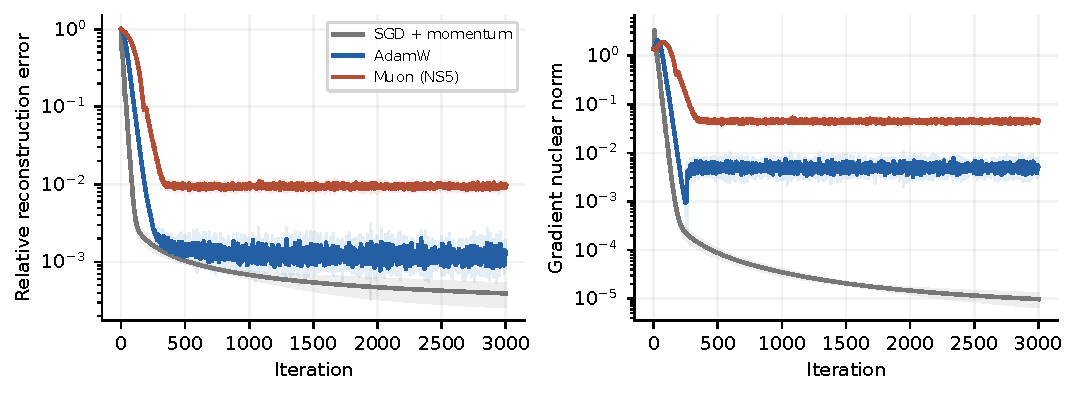
\includegraphics[width=\linewidth]{fig1.pdf}
\caption{非凸病态矩阵分解：相对重构误差与真实梯度核范数。曲线为三个种子的均值，阴影为样本标准差；两图均用对数纵轴。}\label{fig:factorization-new}
\end{figure}

本次矩阵分解中，普通动量 SGD 获得更低的末点重构误差；Muon 的归一化常步长在末段留下残差。因此，病态目标本身并不构成“Muon 必然加速”的证据。该四次因子目标只有局部光滑性，且存在因子缩放不唯一性，不能不加条件地代入全局光滑定理。附录中的固定二次问题才是与原始理论假设直接对应的受控数值检查。

\subsection{CIFAR-10 与完整 ResNet-18}
CIFAR-10 的官方数据包含 50,000 张训练图和 10,000 张测试图\citep{cifar2009}。从官方训练部分按类别分层保留 5,000 张作验证，其余 45,000 张用于训练。划分种子、图像数和索引摘要记录在数据清单中；下载的官方二进制压缩包先核对发布页的 MD5，再解析像素，不反序列化 pickle。

模型严格采用 ResNet-18 的 $[2,2,2,2]$ 基本块结构与 $[64,128,256,512]$ 通道宽度\citep{resnet2016}，保留原始 $7\times7$、步长 2 的输入卷积及 max-pool，只把分类层改为 10 类，共 11,181,642 个参数。输入使用原始 $32\times32$ 图像；这与常见的 $3\times3$ stem CIFAR 变体不同，空间分辨率下降更早。所有方法使用相同结构，不与采用另一种 stem 的公开准确率作直接比较。

训练增强为四像素补零、随机裁剪与水平翻转，再按固定通道均值和标准差归一化。批量 128，正式训练 3 个 epoch，共 1056 次更新，前 50 步预热，之后余弦下降到初始学习率的 0.1 倍。本实验是完整数据上的短程 GPU 比较，不能据此推断充分训练后的最终准确率。

\begin{table}[htbp]\centering\footnotesize
\caption{固定超参数与硬件设置。偏置和归一化参数均不衰减；SGD 使用耦合 L2，两个自适应配置使用解耦衰减。}\label{tab:cifar-config}
\resizebox{\linewidth}{!}{\begin{tabular}{lccc}\toprule
配置项 & SGD+M & AdamW & Muon 混合 \\ \midrule
模型 / 参数量 & \multicolumn{3}{c}{完整 ResNet-18 / 11,181,642} \\
输入 / stem & \multicolumn{3}{c}{$32\times32$ / 原始 $7\times7$、步长 2，保留 max-pool} \\
训练 / 验证 / 测试 & \multicolumn{3}{c}{45,000 / 5,000 / 10,000} \\
批量 / epoch / 种子 & \multicolumn{3}{c}{128 / 3 / 0、1、2} \\
硬件 / 精度 & \multicolumn{3}{c}{单张 H20-3e，Xeon 6759P-C；float32、4 个 CPU 线程} \\
共享资源限制 & \multicolumn{3}{c}{GPU 分配器上限 4\%，协作占空目标 35\%，TF32 关闭} \\
选定学习率 & 0.03 & 0.003 & 0.05 \\
动量 / 矩参数 & $0.9$ & $(0.9,0.95)$ & $0.95$；辅助 AdamW $(0.9,0.95)$ \\
矩阵权重衰减 & $5\times10^{-4}$ & $5\times10^{-4}$ & $5\times10^{-4}$ \\
调度 / 调参预算 & \multicolumn{3}{c}{50 步预热、余弦衰减；各 3 个 LR、种子 42、96 步} \\
\bottomrule\end{tabular}
}
\end{table}

图像分类的 SGD、AdamW 与 Muon 学习率候选分别为 $\{0.03,0.1,0.3\}$、$\{0.0003,0.001,0.003\}$、$\{0.005,0.02,0.05\}$。各候选以种子 42 运行 96 步，使用完整验证集的交叉熵选择；辅助 AdamW 固定采用已选定的 AdamW 学习率。有限的短程候选搜索可能偏好早期表现较好的设置，这是协议的限制，不能将其描述为充分调参后的优化器排名。

每个 epoch 在验证集评价并保存检查点。全部训练结束后，才离线计算各 epoch 的测试指标以绘制曲线；检查点选择只使用验证交叉熵。三种主配置共 9 次正式训练，同一模型中其他训练规则不变。ReLU、BatchNorm 及按 epoch 无放回打乱的数据顺序均未被证明满足前述理论的全部条件；该实验报告实际应用结果，不充当定理假设的验证。

\begin{figure}[htbp]\centering
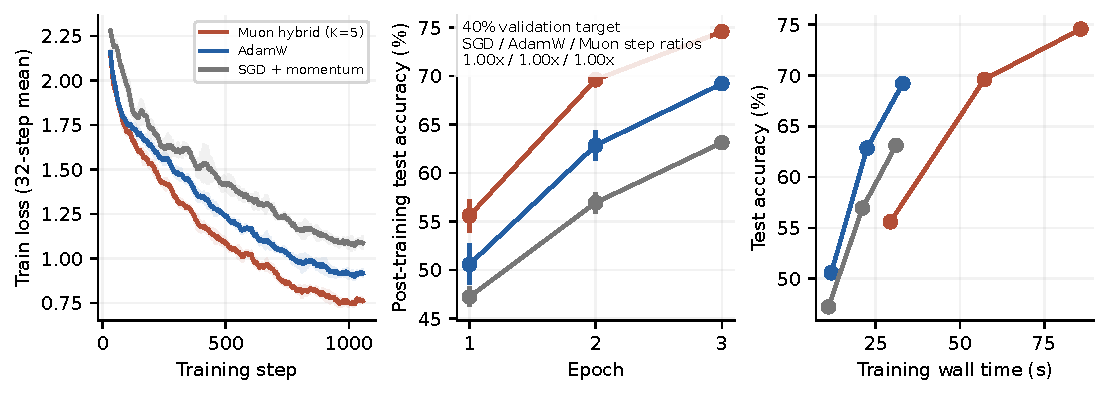
\includegraphics[width=\linewidth]{fig2.pdf}
\caption{CIFAR-10 短程训练。左图训练损失采用 32 步滑动平均；中图为训练后离线测试准确率，误差棒为三个种子的样本标准差；右图横轴包含实际训练、验证、谱诊断及主动等待，不包含后验测试与进程启动。图中步数比使用验证集 40\% 阈值，不能由测试曲线反向选阈值。}\label{fig:cifar-dynamics}
\end{figure}

达标阈值预先固定为验证准确率 40\%，只在 epoch 末检查。达标步数因此具有 352 步的分辨率；没有达到阈值时记为未达标，不用总预算代替首次达标步数。“步数比”定义为同种子 SGD 达标步数除以该方法达标步数；仅在两者均达标时计算，三对结果不全可用时不报告一个掩盖失败样本的平均加速比。

\begin{table}[htbp]\centering\footnotesize
\caption{CIFAR-10 三种子结果。准确率来自验证损失选定的检查点；步数比只衡量样本效率。单步耗时为 CUDA 同步后的活跃时间中位数，不含主动等待。RSS 为独立进程峰值，显存为 PyTorch 峰值已分配量，不含 CUDA 上下文；缓存保留量另存原始日志。}\label{tab:cifar-performance}
\setlength{\tabcolsep}{3pt}
\resizebox{\linewidth}{!}{\begin{tabular}{lccccccc}\toprule
方法 & 末轮 Loss & Acc / \% & 达标步数 & 步数比 & ms/step & RSS / MiB & 显存 / MiB \\ \midrule
SGD+M & $1.136\pm0.010$ & $63.12\pm0.39$ & $352\pm0$ & $1.0\pm0.0$ & $9.3\pm0.0$ & $1523\pm0$ & $254\pm0$ \\
AdamW & $0.957\pm0.012$ & $69.21\pm0.11$ & $352\pm0$ & $1.0\pm0.0$ & $9.9\pm0.0$ & $1594\pm0$ & $295\pm0$ \\
Muon 混合 & $0.798\pm0.008$ & $74.57\pm0.27$ & $352\pm0$ & $1.0\pm0.0$ & $26.8\pm0.2$ & $1618\pm0$ & $255\pm0$ \\
\bottomrule\end{tabular}
}
\end{table}

本次 SGD+M、AdamW 与 Muon 混合配置的选定测试准确率均值分别为 \CifarSGDAcc\%、\CifarAdamAcc\% 与 \CifarMuonAcc\%；对应单步耗时中位数的种子均值为 \CifarSGDStep、\CifarAdamStep\ 和 \CifarMuonStep\ 毫秒。图\ref{fig:cifar-dynamics}与表\ref{tab:cifar-performance}分别呈现按步数和实际时间评价的结果；二者不必给出相同排序。

本次 Muon 的准确率更高，单步活跃时间也更长。三种方法的三个种子均在首次 epoch 检查时达到 40\% 验证阈值，配对步数比均为 1，因此该阈值没有检测到步数优势。这也说明较低阈值与较粗的检查间隔会限制加速指标的区分能力。

\subsection{更新矩阵奇异值谱与机理边界}
选择固定的隐藏卷积参数 \texttt{layer1.0.conv2.weight}，展平为 $64\times576$ 矩阵，记录第 1 步与每个 epoch 末的真实权重差 $\Delta W_t=W_t-W_{t+1}$。该量包含实际优化器方向及权重衰减。各方法使用同一参数层和检查时刻，不挑选谱图更好看的层。归一化谱为 $s_i/s_1$；有效条件数只使用超过 $\max(10^{-6}s_1,10^{-12})$ 的奇异值，并同时保存数值秩。

\begin{figure}[htbp]\centering
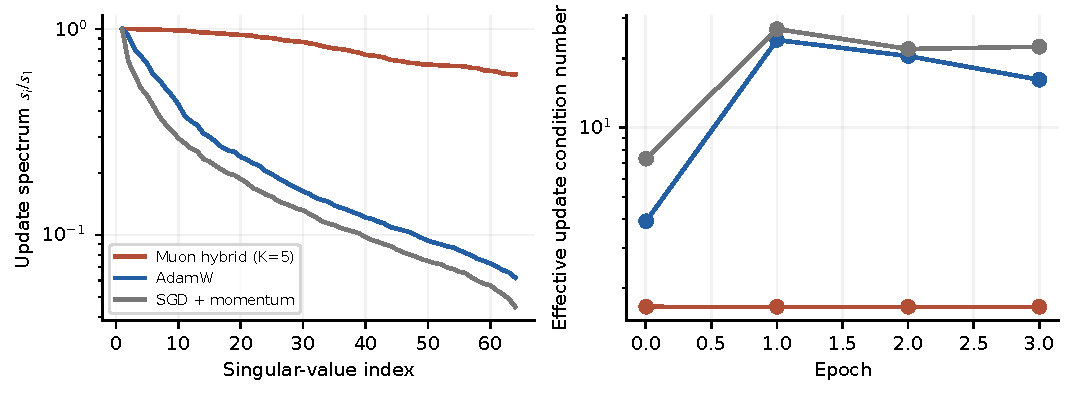
\includegraphics[width=\linewidth]{fig3.pdf}
\caption{代表层实际更新的谱。左图使用末次更新的归一化奇异值，再跨种子平均；右图为预先规定容差下的有效条件数。观察对象是权重更新，不能由此证明激活特征坍缩被消除。}\label{fig:update-spectrum}
\end{figure}

对精确极因子，非零支撑上的奇异值均为 1，这个代数事实解释了谱均衡机制。实际五步多项式、动量、衰减和浮点差分共同影响记录到的更新谱。条件数变小只能说明该更新的谱更均衡；表示层特征是否退化还需要激活协方差、表示秩等额外测量，不能用一幅更新谱图代替。

\subsection{\texorpdfstring{$K=0,1,3,5,7$}{K=0,1,3,5,7} 的训练消融}
对五个 $K$ 值各运行三个种子，共 15 次 Muon 训练，其中 $K=5$ 与主比较共享记录，因此图像分类正式训练总数为 21 次。消融固定 $K=5$ 试跑所选的学习率、辅助 AdamW、初始化、数据增强和训练预算，仅改变多项式次数。$K=0$ 表示仅做 Frobenius 归一化，仍有动量和非零更新。

\begin{figure}[htbp]\centering
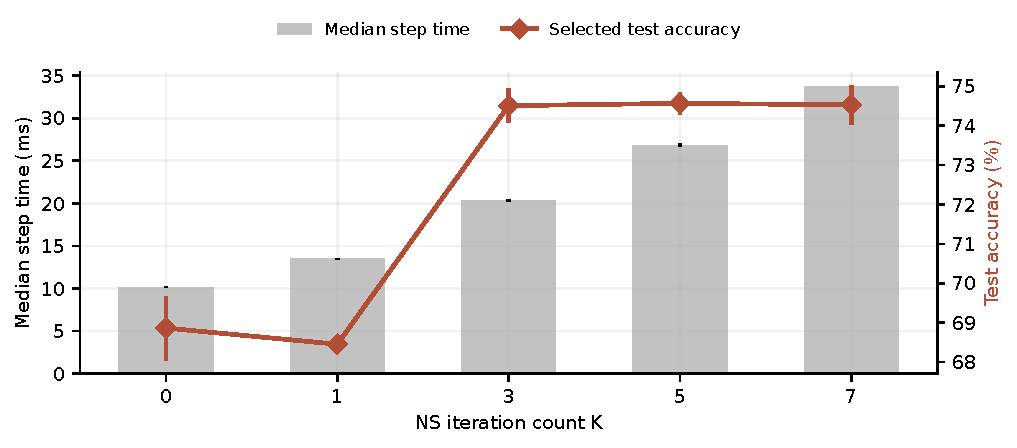
\includegraphics[width=.95\linewidth]{fig4.pdf}
\caption{固定其他设置的 NS 深度消融。柱为单步耗时中位数，线为验证集选定检查点的测试准确率，误差棒为样本标准差。双轴用于展示权衡，不预先指定 $K=5$ 是最佳点。}\label{fig:k-ablation}
\end{figure}

本次末轮验证准确率均值最高的 $K$ 为 \CifarBestValK，详细数值见附录。它仅是本协议中的观测最大值；不同 $K$ 没有分别重调学习率，三个种子也不足以建立普遍最优性结论。代表层同时记录了采样时刻的 $\|O_t-O_t^\star\|_2$，便于核查近似程度，但这些有限检查点不是式\eqref{eq:delta-assumption}的全程误差证书。

从本次样本均值看，$K=3$ 以更低的单步成本取得接近 $K=5$ 的测试准确率；$K=7$ 的末轮验证均值最高，却没有带来更高的选定测试均值。这些差异仍需结合三个种子的波动解释，不能单独据此确定普遍最优的迭代深度。

还有一个重要的机理限制：$K=0$ 的前置归一化使更新的 Frobenius 长度接近 1，而增加多项式次数也会改变更新幅度。因此，固定学习率的 $K$ 消融同时包含幅度和方向的影响，不能把准确率差全部归因于正交化质量。若要进一步分离两者，还需另做 RMS 匹配或更新范数匹配实验。
\FloatBarrier

\section{结论}
Muon 的精确方向可由谱范数单位球上的线性最小化解释，矩阵核范数自然出现在下降量中。通过动量误差递推，本文在同一框架内得到确定性 $O(T^{-1/2})$ 与固定批量随机 $O(T^{-1/4})$ 的平均梯度范数上界，并保留维度、噪声及初始目标差的依赖。这些结果说明在明确假设和参数调度下，归一化矩阵更新能够接近一阶平稳点，而非证明任意实用配置都会收敛到全局最优解。

在此基础上，本文补充了显式依赖谱范数近似误差的条件定理。统一的误差界 $\delta<1$ 使相对误差可吸收入下降项，但固定五步 NS 并不自动保证这一条件。实用混合版本的收敛仍需要与其 Nesterov、衰减和辅助参数组相匹配的联合分析。

新增实验中，病态矩阵分解没有显示 Muon 的普遍优势；CIFAR-10 同时给出三种子准确率、达标步数、H20 单步活跃时间与显存开销。共享服务器采用主动等待，墙钟反映本次资源策略而非独占设备吞吐量。更新谱只解释方向结构，不能直接推断表示特征坍缩；$K$ 消融展示本次观测到的权衡，不把 $K=5$ 预设为最优。后续可延长训练预算、增加随机种子，并研究动态步长、非光滑激活下的分析以及分布式通信成本。完整日志和公开版本使上述结论可以被复查。

\section{代码与复现说明}\label{sec:reproduce}
公开仓库：\url{https://github.com/TrueEway/muon-course-project/tree/v1.1}。本次提交使用 \texttt{v1.1}，历史标签 \texttt{v1.0} 保持不变。新增原始记录集合摘要前 16 位为 \texttt{\RevisionDigest}；完整摘要位于 \path{output/revision_audit.json}。源码、环境、数据校验值、CSV/JSON/NPZ 和独立绘图入口均随版本保存。

新增图像训练需要 Linux CUDA 环境。先按当前负载设置 \texttt{MUON\_GPU} 与 \texttt{MUON\_CPUSET}，分别指定一张 GPU 与四个逻辑核，复用已验证的 CUDA PyTorch。在项目根目录执行：
\begin{quote}\small\ttfamily
bash scripts/run\_h20.sh -m experiments.factorization\\
bash scripts/run\_h20.sh train.py\\
bash scripts/finalize\_h20.sh
\end{quote}
最后一条命令从完整日志绘图，按 XeLaTeX、BibTeX、XeLaTeX、XeLaTeX 的顺序编译，再校验和渲染，得到 \texttt{Muon\_Report.pdf}。完整顺序入口为 \path{scripts/reproduce_h20.sh}，Windows 的构建脚本也可重新编译已有图表。配置一致的单次实验会跳过；重跑应使用独立副本，保留冻结记录。历史 CPU 协议、依赖及命令另见仓库 README，不与新版 GPU 时间混用。

\clearpage
\bibliographystyle{unsrtnat}
\bibliography{references}
\clearpage
\appendix
\section{边界情形与证明核查}
新增检查包括完整 ResNet-18 的参数量与八个残差块、卷积参数组的无重复覆盖、$K=0$ 的准确含义和零梯度行为、谱范数误差下降不等式的数值核查、两因子目标的联合有限差分梯度，以及数据增强的种子复现。它们补充下文原有版本的检查项目。
\subsection{新增实验的数值汇总}
\begin{table}[htbp]\centering\small
\caption{新增病态矩阵分解的末点指标，三个种子的均值与样本标准差。}
\begin{tabular}{lcc}\toprule
方法 & 末点目标值 & 相对重构误差 \\ \midrule
SGD + momentum & $1.83\times10^{-7}\,\pm\,1.1\times10^{-7}$ & $3.91\times10^{-4}\,\pm\,1.3\times10^{-4}$ \\
AdamW & $2.89\times10^{-6}\,\pm\,2.4\times10^{-6}$ & $1.52\times10^{-3}\,\pm\,6.4\times10^{-4}$ \\
Muon (NS5) & $1.02\times10^{-4}\,\pm\,2.7\times10^{-5}$ & $9.49\times10^{-3}\,\pm\,1.3\times10^{-3}$ \\
\bottomrule\end{tabular}

\end{table}
\begin{table}[htbp]\centering\small
\caption{ResNet-18 的 $K$ 消融数值。学习率固定为 $K=5$ 试跑选定值，其余训练设置完全相同。}
\begin{tabular}{cccc}\toprule
$K$ & 末轮验证 Acc / \% & 选定测试 Acc / \% & ms/step \\ \midrule
0 & $69.440\,\pm\,0.801$ & $68.863\,\pm\,0.811$ & $10.166\,\pm\,0.083$ \\
1 & $68.927\,\pm\,0.814$ & $68.453\,\pm\,0.186$ & $13.484\,\pm\,0.047$ \\
3 & $75.580\,\pm\,0.208$ & $74.507\,\pm\,0.430$ & $20.316\,\pm\,0.104$ \\
5 & $75.420\,\pm\,0.517$ & $74.567\,\pm\,0.271$ & $26.846\,\pm\,0.216$ \\
7 & $75.633\,\pm\,0.244$ & $74.527\,\pm\,0.485$ & $33.671\,\pm\,0.059$ \\
\bottomrule\end{tabular}

\end{table}
\subsection{一个不应使用的矩阵范数不等式}
对可逆对角矩阵 $S=\operatorname{diag}(1,2)$，
\begin{equation}
 \op{S^{-1}}=1,\qquad \frac1{\op S}=\frac12.
\end{equation}
因此一般不能使用 $\|S^{-1}\|_{\mathrm{op}}\leq1/\|S\|_{\mathrm{op}}$。正确关系是 $\|S^{-1}\|_{\mathrm{op}}=1/s_{\min}(S)$。本文用式\eqref{eq:alignment}替代含逆矩阵的论证，同时避免要求梯度或动量始终满秩。指出这一中间步骤的问题，不等于断言所有相关定理都无法通过其他方法证明。

\subsection{数值秩与浮点误差}
精确数学定义只保留正奇异值。程序采用阈值
\begin{equation}
 s_i>\max(m,n)\,\epsilon_{\mathrm{mach}}\,s_1,
\end{equation}
以避免浮点 SVD 把数值零误认为有效方向。因此实现严格说是数值秩上的极因子。合成实验使用 float64；语言模型的 SVD 对照使用 float32。阈值附近的方向可能与实数模型不同，这是实现限制，不能通过把容差设置为零来消除。

\subsection{检查项目与实验解释}
单元检查包括：零秩、秩一与满秩矩阵上的对偶恒等式和范数界；二次目标的有限差分梯度；带任意跟踪误差的单步下降；有限多项式与标量奇异值迭代的一致性；更新时不原地改写梯度；参数分组无重复且覆盖全部参数；因果注意力不使用未来字符；同一种子训练一步的精确复现。

有限步定理控制的是理论期望，随机实验只提供有限样本观察。随机实验的 CSV 内包含真实梯度，是因为合成目标允许计算该量；这并不意味着实际大模型训练时已知全数据梯度。语言模型没有验证全局光滑性或全程方差界，故其曲线只能作为应用实验报告。

\section{运行配置与文件对应}
\begin{table}[htbp]\centering\small
\caption{主要运行记录及其用途}
\begin{tabularx}{\linewidth}{lX}\toprule
记录目录或文件 & 内容 \\\midrule
\texttt{output/results/deterministic} & 每个种子、条件数、预算与方法的逐步 CSV 及配置 JSON \\
\texttt{output/results/stochastic} & 噪声、批量、预算、真实梯度与动量误差 \\
\texttt{output/results/orthogonalization} & 各形状、输入谱、步数的误差与重复计时 \\
\texttt{output/results/language/pilot} & 全部候选学习率的试跑记录 \\
\texttt{output/results/language/formal} & 正式训练及测试指标，检查点步数和参数分组 \\
\texttt{data/manifest.json} & 固定数据链接、提交版本、SHA256、词表与划分大小 \\
\texttt{output/audit.json} & 运行计数、数值核查和结果记录集合校验值 \\
\bottomrule\end{tabularx}
\end{table}
正式检查点保存在本地输出目录，不纳入 GitHub 原始记录集合；复现脚本可以重新训练得到。计时相关字段会随机器负载变化，因而重新运行后的结果集合 SHA256 也会变化。校验值用于标识本次提交的记录集合，不要求不同机器重跑后具有相同的时间戳、耗时或集合摘要。

历史结果集合摘要为 \texttt{\ResultDigest}。附录语言模型使用的 Tiny Shakespeare 文件 SHA256 为
\begin{center}\footnotesize\ttfamily\expandafter\nolinkurl\expandafter{\DataSHA}\end{center}

\subsection{理论与实现的对照表}
\begin{table}[htbp]
\centering\small
\caption{理论版本与语言模型实现的对应关系}
\begin{tabularx}{\linewidth}{lXX}
\toprule 项目 & 理论与矩阵实验 & 语言模型实验 \\\midrule
正交化 & 精确紧致极因子 & 精确极因子或五步多项式 \\
动量初始化 & $M_1=G_1$ & 缓冲区初始化为零 \\
Nesterov / 形状缩放 & 均不使用 & 两种 Muon 配置均使用 \\
权重衰减 & 0 & 权重矩阵 0.01 \\
其他参数 & 单个矩阵 & AdamW 辅助参数组 \\
步长与动量 & 按定理设置 & 验证集选步长，$\beta=0.95$ \\
\bottomrule
\end{tabularx}
\end{table}

\section{v1.0 补充实验与原始记录}\label{sec:legacy-experiments}
本附录保存 2026 年 11 月 20 日版本的实验。以下硬件线程数、运行总数和“全部实验”均指该历史协议；新增 ResNet-18 与矩阵分解结果采用正文中的 v1.1 协议。原始数值记录未因本轮增补而重写。
\subsection{公共协议与可重复性}
全部实验在 Windows 11、Intel Core Ultra 5 225H、约 32 GB 内存的本机上执行，采用 Python 3.12.14、NumPy 2.5.5 与 PyTorch 2.15.0+cpu。正式随机种子为 $0,1,2$，学习率选择种子为 42。原始记录保存每一步指标，汇总表给出三个种子的均值与样本标准差（分母为 $n-1$）。只有三个重复时，误差棒仅描述这三次运行的波动，不作总体显著性判断。

矩阵实验采用 NumPy float64，BLAS 固定单线程；语言模型采用 PyTorch float32，正式运行固定两个计算线程，并启用确定性算法。CPU 微基准分别记录 1、2、4 线程，正式实验始终使用统一的双线程设置。随机数据、初始化与训练批次分别由固定种子生成。计时使用单调高精度时钟，仍可能受操作系统调度与 CPU 频率影响。

本次包含 144 次确定性矩阵运行、48 次随机矩阵运行、108 条正交化配置测量、9 次语言模型试跑和 9 次正式语言模型训练。所有合成目标的权重衰减均为零。理论界用于期望量；把三个种子的实测平均画在理论界旁边是数值核对，不构成概率保证或数学证明。

\subsection{确定性矩阵二次问题}
构造
\begin{equation}\label{eq:synthetic}
 f(W)=\frac12\|A(W-W^\star)\|_F^2,
 \quad W\in\R^{32\times16},\quad A\in\R^{32\times32}.
\end{equation}
$A$ 的左右奇异向量由高斯矩阵 QR 分解产生，奇异值从 1 到 $\kappa^{-1/2}$ 按几何间隔排列。因此 $L=\op{A^\top A}=1$，Hessian 条件数恰为 $\kappa\in\{1,10,100\}$，目标下界为 0。初始位移归一化为 Frobenius 范数 1，各方法共享同一问题和初值。

比较梯度下降（步长 0.9）、EMA 动量梯度下降（$\beta=0.9$，步长 0.1），以及 $\beta=0$ 和 0.9 的精确 Muon。Muon 按 $\eta=0.1T^{-1/2}$ 设置步长，分别运行 $T=100,300,1000,3000$。基线步长是已知 $L=1$ 后的固定设置，不代表分别充分调参后的性能上限，也不用于声称公平的最优算法排名。

\begin{figure}[htbp]\centering
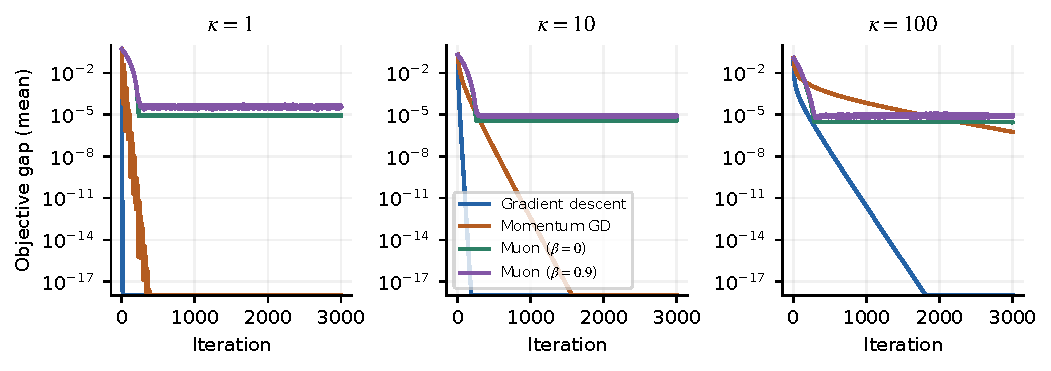
\includegraphics[width=\linewidth]{deterministic_loss.pdf}
\caption{确定性二次目标，$T=3000$。曲线为三个种子的目标差均值，绘图下限为 $10^{-18}$，因此底部截断不表示精确达到零。归一化更新与固定步长基线的运行方式不同，比较时需结合正文中的步长设置。}\label{fig:detloss}
\end{figure}

\begin{table}[htbp]\centering\small
\caption{$\kappa=10,T=3000$ 的确定性结果。末点目标差对应 $W_{T+1}$；平均梯度使用 $W_1,\ldots,W_T$。}
\begin{tabular}{lcc}\toprule
方法 & 末点目标差 & 平均梯度核范数 \\ \midrule
Gradient descent & $1.21\times10^{-32}\,\pm\,1.1\times10^{-33}$ & $0.002\,\pm\,0.000$ \\
Momentum GD & $1.79\times10^{-30}\,\pm\,7.6\times10^{-32}$ & $0.011\,\pm\,0.000$ \\
Muon ($\beta=0$) & $3.72\times10^{-6}\,\pm\,2.6\times10^{-7}$ & $0.046\,\pm\,0.002$ \\
Muon ($\beta=0.9$) & $7.56\times10^{-6}\,\pm\,9.9\times10^{-7}$ & $0.046\,\pm\,0.002$ \\
\bottomrule\end{tabular}

\label{tab:det}
\end{table}

梯度下降在低条件数二次问题上可以迅速降低目标值，说明这种问题并不是用来展示 Muon 全面优势的任务。Muon 的归一化方向在梯度变小后仍保留有限更新长度，因此常步长末段可能出现残差或振荡；动量也会使更新方向滞后于当前梯度。图\ref{fig:detrate}改变预算及相应步长，评价与定理一致的全程平均梯度，而非仅比较末点目标值。

\begin{figure}[htbp]\centering
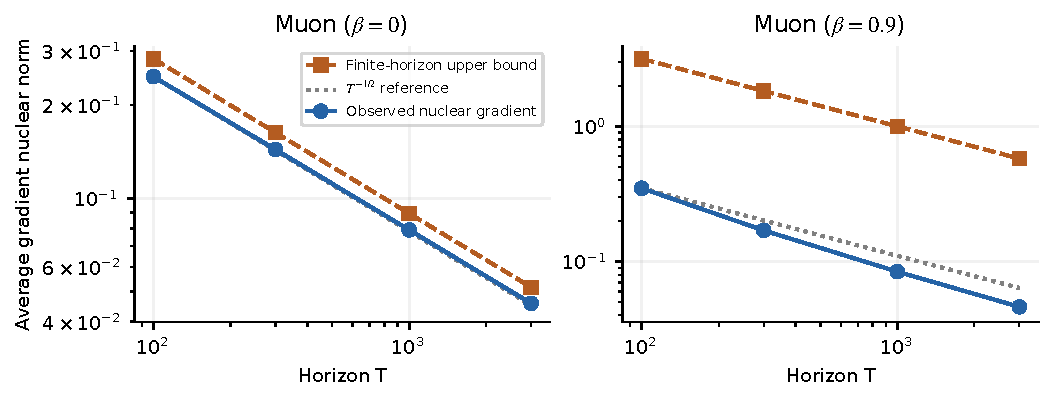
\includegraphics[width=\linewidth]{deterministic_rate.pdf}
\caption{$\kappa=10$ 下的预算实验。误差棒为样本标准差，虚线为显式有限步上界，点线仅为经过首个实测点的 $T^{-1/2}$ 参考线。}\label{fig:detrate}
\end{figure}

跟踪误差的通用估计使用了 $\sqrt r$ 与几何级数上界，因而非零动量下的理论常数可能相当保守。实验检查每一步式\eqref{eq:descent}，最大正向违反量为 \texttt{\MaxDescentViolation}，处于浮点舍入量级；这是实现与推导的一致性检查，不能替代前面的证明。

\subsection{已知方差的随机梯度问题}
固定 $\kappa=10$，使用
\begin{equation}\label{eq:oracle}
 G_t=\nabla f(W_t)+\frac{\sigma}{\sqrt{Bmn}}\Xi_t,
 \qquad (\Xi_t)_{ij}\overset{\mathrm{iid}}\sim\mathcal N(0,1).
\end{equation}
所以 $\E[G_t\mid\mathcal F_t]=H_t$ 且 $\E\|G_t-H_t\|_F^2=\sigma^2/B$。程序直接采样与 $B$ 个独立高斯噪声平均同分布的噪声，不实际计算 $B$ 次样本损失；因此这里只检验方差与梯度调用模型，不报告批量计算加速。

取 $\sigma\in\{0.01,0.1\}$、$B\in\{1,16\}$ 和 $T\in\{256,1024,4096,16384\}$，采用式\eqref{eq:schedule}及 $c=0.1$。每一步同时记录真实梯度、目标值和 $\|M_t-H_t\|_F$。真实梯度仅用于评价，优化更新只接触带噪声的 $G_t$。

\begin{figure}[htbp]\centering
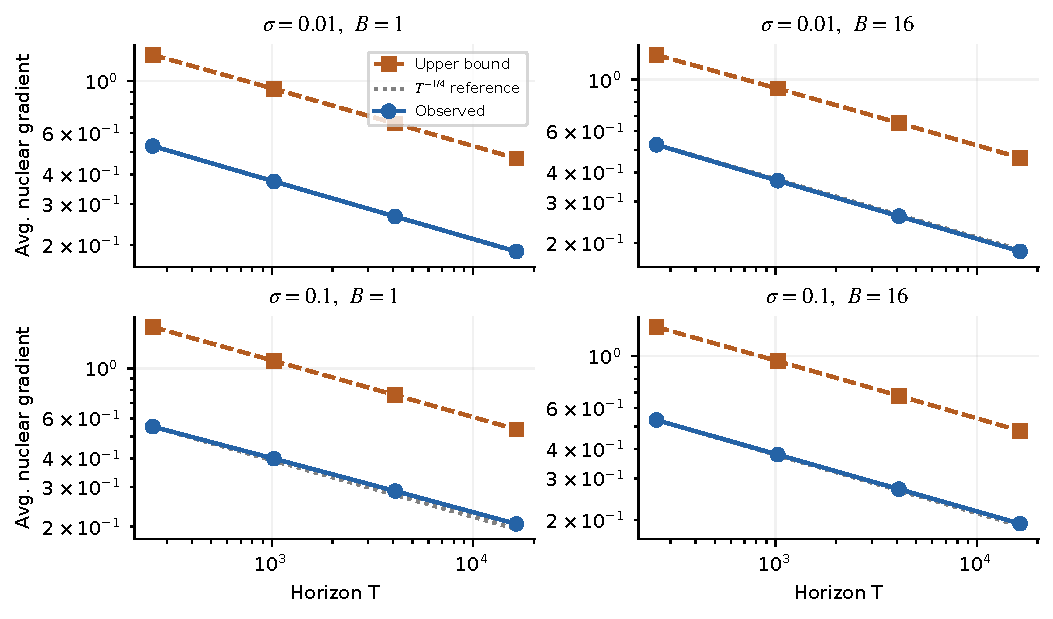
\includegraphics[width=0.96\linewidth]{stochastic_rate.pdf}
\caption{随机矩阵实验的全程平均梯度核范数。理论上界按同一问题的 $L,r,\Delta,\sigma,B$ 计算。灰色参考线没有进行曲线拟合。}\label{fig:stochastic}
\end{figure}

\begin{table}[htbp]\centering\small
\caption{$T=16384$ 的随机实验；全部数值为三个种子的均值与样本标准差。}
\begin{tabular}{ccccc}\toprule
$\sigma$ & $B$ & 平均梯度核范数 & 有限步界 & 平均跟踪误差 \\ \midrule
0.01 & 1 & $0.188\,\pm\,0.010$ & $0.468\,\pm\,0.010$ & $0.006\,\pm\,0.000$ \\
0.01 & 16 & $0.184\,\pm\,0.010$ & $0.462\,\pm\,0.010$ & $0.005\,\pm\,0.000$ \\
0.1 & 1 & $0.206\,\pm\,0.010$ & $0.537\,\pm\,0.010$ & $0.013\,\pm\,0.000$ \\
0.1 & 16 & $0.192\,\pm\,0.010$ & $0.480\,\pm\,0.010$ & $0.008\,\pm\,0.000$ \\
\bottomrule\end{tabular}

\label{tab:stochastic}
\end{table}

批量和噪声水平只改变误差分解中的随机部分，漂移部分仍由步长和动量共同决定。对这一强凸二次目标，实测下降可以快于一般非凸理论的最坏上界，也可能在有限预算中尚未进入渐近阶段。因此，图\ref{fig:stochastic}用于展示预算变化与界的保守程度，不把几个点的斜率当作收敛阶数的证明。全部精确 Muon 确定性和随机运行中，单次实测平均梯度与相应期望上界之比的最大值为 \MaxBoundRatio；随机样本不超界是本次结果，而非定理所要求的逐样本性质。

\subsection{有限步正交化的谱敏感性}
分别构造 $32\times32$、$64\times16$、$16\times64$ 矩阵。平坦谱的所有奇异值均为 1；病态谱从 1 到 $10^{-6}$ 按几何间隔排列；秩亏谱再把后一半奇异值置零。每个形状、谱和种子均测量 1、3、5、10 步 Newton--Schulz。精确极因子和多项式采用相同的紧致支撑约定。

\begin{figure}[htbp]\centering
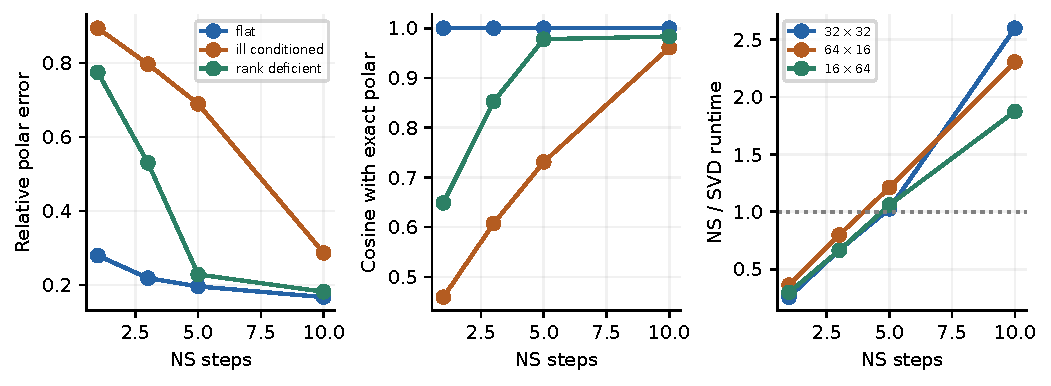
\includegraphics[width=\linewidth]{orthogonalization.pdf}
\caption{有限多项式的相对极因子误差、方向余弦和 CPU 耗时比。前两图跨形状与种子平均；右图跨谱与种子平均，每个计时重复 30 次。}\label{fig:ns}
\end{figure}

\begin{table}[htbp]\centering\small
\caption{五步 Newton--Schulz 与精确极因子的差异，跨三个形状和三个种子汇总。}
\begin{tabular}{lcc}\toprule
输入谱 & 相对 Frobenius 误差 & 方向余弦 \\ \midrule
平坦谱 & $0.197\,\pm\,0.133$ & $1.000\,\pm\,0.000$ \\
病态谱 & $0.690\,\pm\,0.003$ & $0.731\,\pm\,0.004$ \\
秩亏谱 & $0.229\,\pm\,0.009$ & $0.978\,\pm\,0.003$ \\
\bottomrule\end{tabular}

\end{table}

病态谱中的很小奇异值经过有限次多项式后仍可能远离 1，所以相对极因子误差与平坦谱明显不同。误差较大不等于该方向对目标必然无效：极因子误差对各支撑方向一视同仁，而真正的下降量是当前梯度与更新方向的内积。图\ref{fig:ns}同时报告方向余弦，以避免仅凭一个误差指标解释训练效果。此处矩阵尺寸很小、采用 CPU float64，计时比不能外推为 GPU 上大矩阵的性能结论。

\subsection{微型 Transformer 语言模型}
使用 Tiny Shakespeare\citep{karpathy2015}，词表包含 \VocabSize\ 个字符。按原始文本顺序划分后，训练、验证、测试集分别包含 \TrainChars、\ValChars、\TestChars\ 个字符，窗口严格限制在各自集合内。词表由整份公开语料的字符集合建立，只涉及字符编码，不用测试集选择模型或超参数。

模型为两层预归一化因果 Transformer\citep{vaswani2017}：宽度 64，4 个注意力头，前馈宽度 256，学习式位置嵌入，上下文 64，批量 16，不使用 dropout，不共享输入输出嵌入。参数总数为 \ParameterCount。两个 Muon 配置均只更新块内 8 个二维权重矩阵，其余参数使用 AdamW；全参数 AdamW 是基线。

先用种子 42 对每种配置分别试跑三个学习率，各训练 300 步，按末次验证交叉熵选取。AdamW 候选为 $\{0.0003,0.001,0.003\}$，Muon 候选为 $\{0.005,0.02,0.05\}$。辅助 AdamW 共享基线选出的学习率 \AdamLR。每种配置恰有三个候选，但这不是对不同优化器的穷尽搜索，也没有声称所有超参数都已最优。

\begin{table}[htbp]\centering\small
\caption{固定种子 42 的学习率试跑，选择依据仅为验证集交叉熵。}
\begin{tabular}{lcc}\toprule
方法 & 学习率 & 300 步验证交叉熵 \\ \midrule
AdamW & 0.0003 & 2.7250 \\
AdamW & 0.001 & 2.4640 \\
AdamW & 0.003 & 2.3875 \\
Muon-SVD+AdamW & 0.005 & 2.3506 \\
Muon-SVD+AdamW & 0.02 & 2.1306 \\
Muon-SVD+AdamW & 0.05 & 2.1332 \\
Muon-NS+AdamW & 0.005 & 2.3599 \\
Muon-NS+AdamW & 0.02 & 2.1497 \\
Muon-NS+AdamW & 0.05 & 2.1288 \\
\bottomrule\end{tabular}

\label{tab:pilot}
\end{table}

正式运行从头初始化，每次训练 1500 步，即处理 1536000 个训练字符目标。前 100 步线性预热，此后余弦下降到初始学习率的 0.1 倍。AdamW 使用 $(\beta_1,\beta_2)=(0.9,0.95)$、$\epsilon=10^{-8}$；Muon 使用 $\beta=0.95$ 和 Nesterov 修正。所有权重矩阵衰减系数为 0.01，偏置与归一化参数不衰减；不使用梯度裁剪。

每 50 步在固定 32 个验证批量上评价，选择验证损失最低的检查点，然后对完整测试划分计算一次交叉熵。测试窗口不重叠，相邻窗口共享一个作为上下文的边界字符，各目标字符除首字符外恰被评价一次。不同方法在相同种子下共享初始化和训练批次顺序。正式方法运行顺序随种子轮换，减少固定顺序对计时的影响。

\begin{figure}[H]\centering
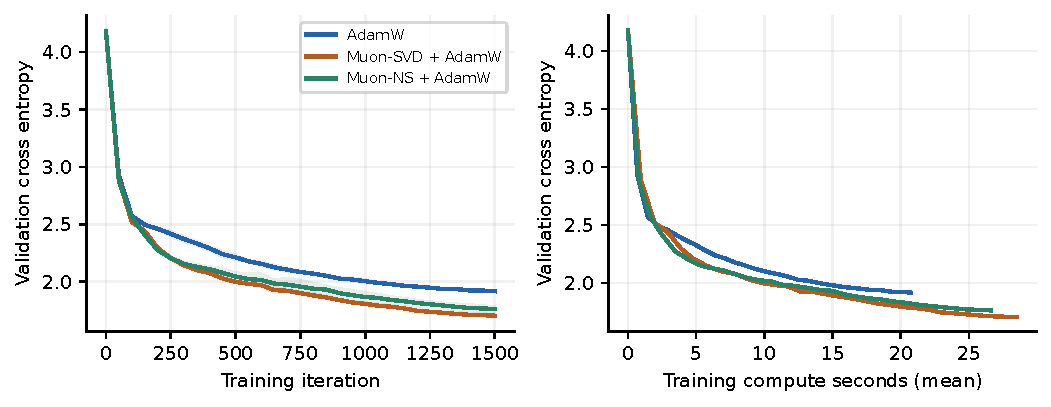
\includegraphics[width=\linewidth]{language_learning.pdf}
\caption{语言模型验证曲线。左图阴影为三个种子的样本标准差；右图把同一步的平均验证损失放在平均训练计算耗时处，并非对相同墙钟时刻插值。训练计算耗时包含采样、前后向传播和更新，不包含验证、测试、数据下载及检查点写入。}\label{fig:lm}
\end{figure}

\begin{table}[H]\centering\small
\caption{微型语言模型正式结果。测试指标来自按验证集选择的检查点；困惑度为 $\exp(\mathrm{CE})$，先对每个种子计算，再汇总。}
\resizebox{\linewidth}{!}{\begin{tabular}{lcccc}\toprule
方法 & 学习率 & 测试交叉熵 & 测试困惑度 & 训练计算耗时 / 秒 \\ \midrule
AdamW & 0.003 & $1.962\,\pm\,0.007$ & $7.110\,\pm\,0.047$ & $20.710\,\pm\,1.841$ \\
Muon-SVD+AdamW & 0.02 & $1.793\,\pm\,0.008$ & $6.008\,\pm\,0.051$ & $28.504\,\pm\,0.781$ \\
Muon-NS+AdamW & 0.05 & $1.843\,\pm\,0.025$ & $6.316\,\pm\,0.156$ & $26.577\,\pm\,0.563$ \\
\bottomrule\end{tabular}
}\label{tab:lm}
\end{table}

本次 AdamW、Muon-SVD+AdamW 与 Muon-NS+AdamW 的测试交叉熵均值依次为 \AdamCE、\SVDCE、\NSCE，训练计算耗时均值依次为 \AdamTime、\SVDTime、\NSTime\ 秒。表\ref{tab:lm}与图\ref{fig:lm}需要同时阅读：较低的按步数损失并不自动对应较少的计算时间。精确 SVD 对照用于隔离正交化方式，其计算代价本来就可能高于有限矩阵多项式。

三种配置共同改变了训练轨迹，混合 Muon 与全参数 AdamW 的比较不能单独识别某个参数组的因果贡献。小字符模型、短上下文、有限训练预算和三个种子也限制了结论范围。这里报告实际测量，不把未达到的固定损失阈值换算为假想加速比，也不把优化过程的定理直接解释为泛化保证。
\FloatBarrier

\end{document}
